\chapter{CMOS MAPS sensors} \label{ch:CMOS}

This chapter introduces the essential features of the semiconductor detector technology, going through the history of its advancements, which have led to the currently most promising sensors based on CMOS logic structure, the Monolithic Active Pixel Sensors (MAPS). The VTX project wants to make the most of technologies that have already proven reliable in precision measurements, obtaining fast readout and high radiation tolerance, like the TJ-Monopix development line. We will briefly present it, mentioning the peculiarities of its prototypes, to understand how they could fulfill the Belle II requirements.


\section{Semiconductor detectors} 

Charged particles can be detected through the measurement of the ionization charge released during their passage through solid, liquid, or gaseous detector. Semiconductors are extensively used as ionization detectors since they are easily available and the readout can be finely segmented leading to excellent spacial resolution. This section provides the basic description of the working principle of semiconductor detectors.\\

Solids can be divided into three categories based on their electrical conductivity: conductors, semiconductors and insulators. 
In a solid state lattice, the constituent atoms have a dense periodic arrangement and the energy levels of some level groups lie energetically so dense (order of meV) that one speaks of \emph{energy bands}, separated from each other by a \emph{band gap}, which represents the distance in energy between them (\textbf{$E_{G}$}, energy gap). The electrical conduction properties of materials are determined by the two highest energy bands, which are the \textbf{valence band (VB)} and the \textbf{conduction band (CB)}; in particular, they depend on the band gap between the two levels and on the band occupation, as we can see in~\autoref{fig:energy_band}.

%The energy levels within the same band are so close that the transitions to unoccupied levels, if they are not completely filled, are easily possible. 

\begin{figure}[h!]
\centering
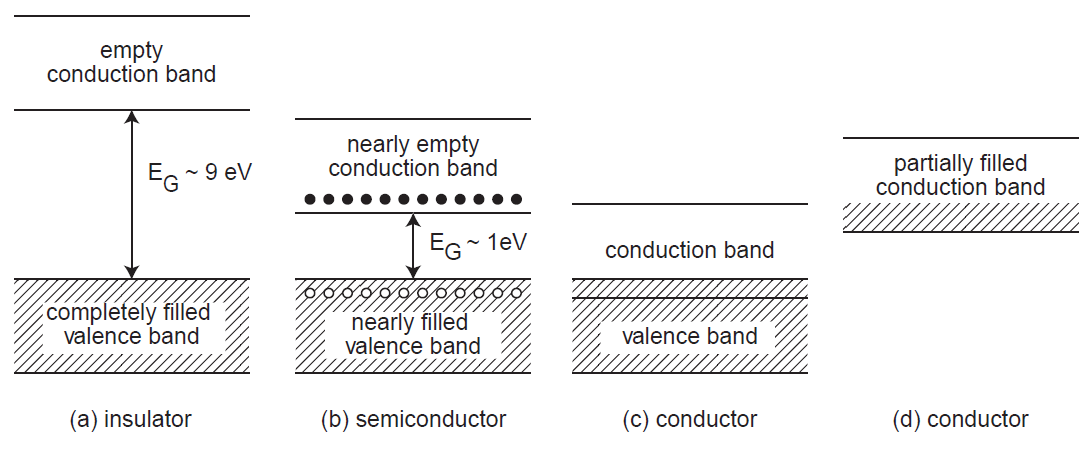
\includegraphics[scale=.6]{energy_band}
\caption{Schematic structure of the energy bands in insulators (a), semiconductors (b) and conductors (c,d).}
\label{fig:energy_band}
\end{figure}

Insulators are characterized by a large energy gap between the VB and CB, of the order of several \unit{eV}, with the number of valence electrons matching the number of states in the VB. Since the band gap is much larger than the thermal excitation energy (KT $\approx$ \SI{25}{meV} at room temperature) the CB is practically empty and the resistivity becomes very large.

Semiconductors have a smaller energy gap with respect to the insulator (for example \SI{1.12}{eV} in silicon). In this way electrons from VB can easily overcome the gap, moving to the CB by thermal excitation or by external electric fields. When an electron makes this transition, it leaves a hole in the VB, which could be filled in turn, by another electrons of the VB. Applying an external electric field, the free electrons in the CB and the holes in the VB start to move producing two different current flows, one with negative carriers and the other with positive carriers.

In conductors, either the conduction and valence bands overlap or the conduction band is partially filled, so transitions within the same band and between the two different bands are easy and current conduction requires minimal energy.


\subsection{Transport of charge carriers and signal formation in semiconductors}

When a charged particle goes through the medium, it releases a certain amount of energy mainly by ionization. Most of this energy loss causes the formation of positive and negative charges. In semiconductors these carriers are the hole-electron pairs created by ionization, which start to move in opposite direction if an external electric field is applied: the holes (positive) migrate towards the \textit{cathode} and the electrons (negative) towards the \textit{anode}, which sense the signal induced by this movement. Their drift induces an accumulation of charges on the electrode surfaces, and it is possible to record this charge induction as a charge, current or voltage signal.\\

The charge carrier density of semiconductors can be modified by doping the material with specific chemical elements, causing also a modification of their conduction properties.
Undoped semiconductors are called \emph{intrinsic semiconductors}. \emph{Extrinsic semiconductors} instead, are artificially doped with external impurities like: 

\begin{itemize}
\item Pentavalent elements (P, As, Sb), called \emph{donors}, added in a tetravalent material (Si, Ge) produce an excess of conduction electrons with respect to the holes (n doping, \autoref{fig:doping} (a)).
\item Trivalent atoms (B, Al, Ga), called \emph{acceptors}, create an excess of holes (p doping, \autoref{fig:doping} (b)).
\end{itemize}

\begin{figure}[h!]
\centering
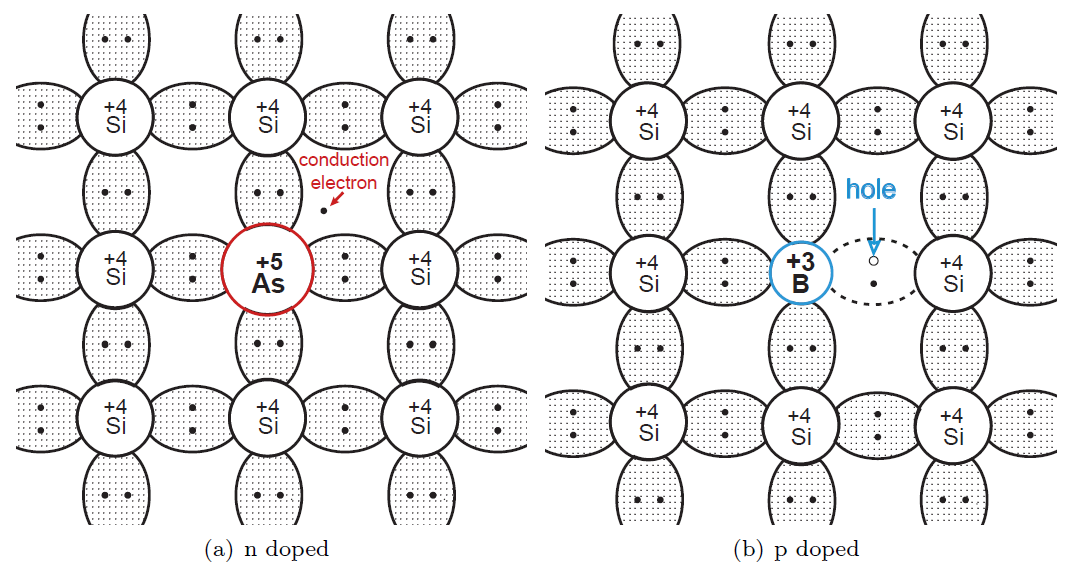
\includegraphics[scale=.5]{doping}
\caption{Schematic representation of atom bonding structure in n-doped and p-doped semiconductors.}
\label{fig:doping}
\end{figure}


\subsection{The pn junctions as detector}

The base material employed in semiconductor detectors is silicon, because it is stable, abundant and it has a low band gap which allows an adequate amount of charge to be produced.\\ 
When a p-doped semiconductor gets in contact with a n-doped material, a \textit{pn junction} is formed. In the p-doped part the holes are the dominant charge carriers, called \textit{majority carriers}, while in the n-doped part, the electrons are dominant. 
The presence of these excesses of opposite charge in the two parts of the junction, generates a density difference across the junction, which causes the diffusion of the majority carriers from each part to the opposite one. At the boundary the charges recombine (that is when a conduction band electron occupies a valence band hole, losing energy), creating a zone which is free of charge carriers, called \textbf{depletion zone}. After the recombination, the atoms of this depletion region are ionized, and so it is no longer neutral, but features a \emph{space-charge} (\autoref{fig:space_charge}): a positive one in the n-layer, and negative in the p-layer. Due to their opposite sign, they generate an intrinsic electric field that stops the original diffusion current.\\

\begin{figure}
\centering
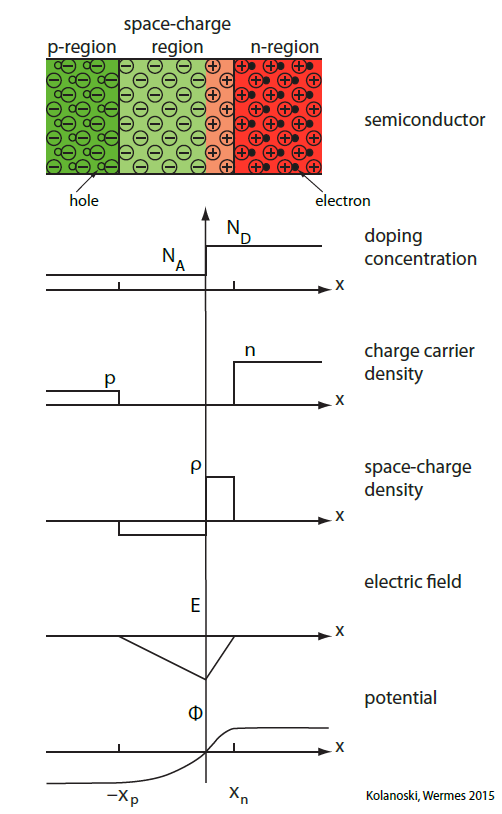
\includegraphics[scale=.6]{pn_junction}
\caption{Doping concentration, charge carrier and space charge densities, electric field strength and electric potential in a pn junction.}
\label{fig:space_charge}
\end{figure}

The application of an external voltage $V_{ext}$ between the two sections of the junction, causes a variation of the depletion region widths, depending on the size and polarity of the applied voltage. It is possible to distinguish:%~\autoref{fig:bias}:

\begin{itemize}
\item \emph{forward bias}, $V_{ext}$>0: a positive external voltage applied to the p side with respect to the n side, causes a reduction of the depletion region;
\item \emph{reverse bias}, $V_{ext}$<0: if a negative voltage at the p side or positive at the n side relative to the respectively opposite side is applied, the depletion region gets wider.
\end{itemize}

The depleted region is a zone without free charge carriers, and with the presence of an external electric field (reverse bias). It is the region where the created charge can be collected and produce a measurable signal.

The basic structure of semiconductor detectors is a reverse biased p-n diode where the depleted region represents the active volume and the diode terminals are the charge collection electrodes.


\section{Hybrid and monolithic pixel sensors}

The collection electrode in semiconductor detectors can be segmented with various patterns by using the features of modern electronics processing technology. Typical detectors have 200-\SI{300}{\micro m} thickness with charge collection time of the order of 5-\SI{10}{ns}, and segmentation of the order of few hundred micron, organized in strips  for 1D measurements or pixels for 2D measurements.

We discuss in more details the \emph{hybrid} and \emph{monolithic} pixel sensors, where the sensor and the readout could be separate entities or integrated on the same silicon substrate \cite{Garcia-Sciveres:2017ymt}.


\subsection{Hybrid pixel detectors}

\textit{Hybrid} pixel detectors are composed by two different parts: a silicon layer structured in pixel cells, and the readout chips with the same cell pattern, that amplify, digitize, store and transmit the hit data. The sensor and the readout are connected at each pixel by a conducting micro-connection (called \emph{bump bond}). In~\autoref{fig:hybrid} an example of a detector module is shown. 
%There are different bonding techniques which allow to connect the two layers, like \emph{bump-bonding}, \emph{flip-chipping} and \emph{3D integration}. 

\begin{figure}[h!]
\centering
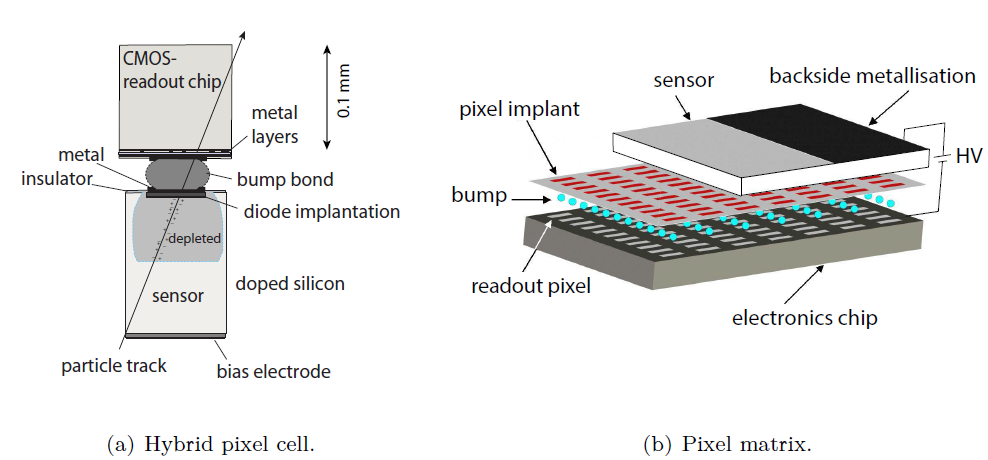
\includegraphics[scale=.6]{hybrid}
\caption{On the left (a), the structure of a single pixel cell, made by the sensor and the electronic readout. On the right (b), an exploiting representation of the entire hybrid pixel matrix arrangement.}
\label{fig:hybrid}
\end{figure}

When a particle crosses the sensor, a signal is generated on the electrodes due to the drift of the charge carriers in the depleted region. This signal passes through the conductive bump in the readout chip, where it is amplified and processed.

The main advantage of the pixel detectors with respect to the strip sensors, is the higher granularity that translates in a lower occupancy, a better signal to noise ratio, and also a better tolerance to radiation damage. The \emph{leakage current} increases as the radiation dose becomes higher, it depends on the volume of the sensors and it is distributed over all the electrode. In pixel detectors this current is shared among more electrodes with respect to the strip detectors, so the leakage current per electrode is smaller. Moreover, as separate entities, sensor and readout could be optimized independently.

Among the disadvantages instead, there are the cost and complexity of the implementation processes, but also larger material thickness, which worsen the track reconstruction and momentum resolution because of the multiple scattering.


\subsection{Monolithic pixel detectors}

We have seen that hybrid detectors are made by the active sensor and the passive readout chip in two separate structures, connected by micro-connections. Since both of them are made of silicon, in principle, it could be possible to build them in a monolithic unit. In this way the amount of material decreases, enhancing the tracking performance and momentum resolution. 

This kind of sensors have been developed either by using dedicated technologies, or by exploiting existing technological processes with minimal modifications. An example of first type is the DEPFET pixel detector, which employs a specifically optimized fabrication process integrating one transistor in each pixel cell.

Developments of the second type have tried to exploit industrial technologies already available, like the CMOS technologies. They have to reach a large depletion zone to improve the signal-to-noise ratio, but also design electrode with small capacitance, to reduce the power consumption and the noise. High radiation tolerance is also required.

Monolithic Active Pixel Sensors (MAPS) employ CMOS technologies to include a readout circuit in their structure and we will see them in more details in~\autoref{sec:MAPS}

\begin{description}
\item[Depleted p-channel field effect transistor (DEPFET)]
\end{description}

In a DEPFET pixel detector, each pixel implements only one transistor. In~\autoref{fig:DEPFET} an example of a DEPFET pixel is shown.

\begin{figure}[h!]
\centering
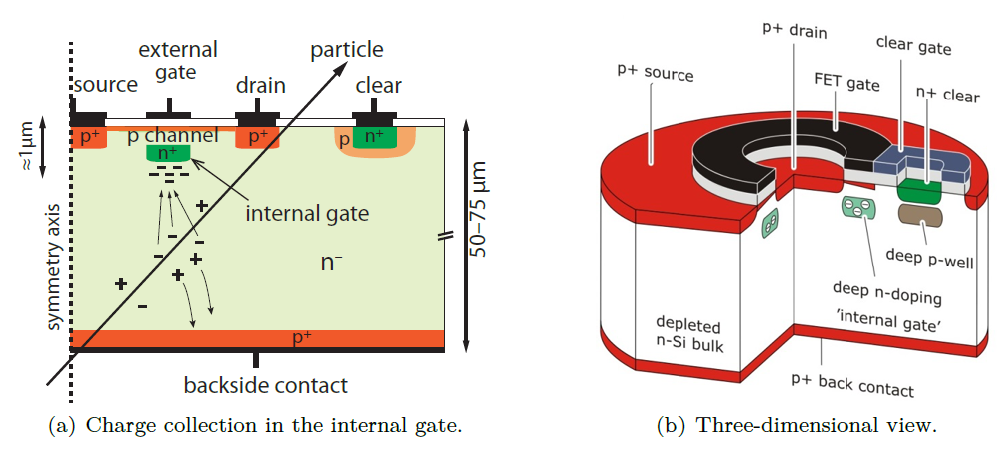
\includegraphics[scale=.6]{DEPFET}
\caption{On the left (a) a cross section of a circular DEPFET pixel cell, where the charge collection is also sketched. On the right (b), a three-dimensional view of the same pixel cell.}
\label{fig:DEPFET}
\end{figure}

The depletion region extends between the backside $p^{+}$ contact and the several $p^{+}$ regions near the transistor element (drain, source and a $n^{+}$ clear contact installed in a \textit{p} region) and the $n^{-}$ substrate. When a traversing particle releases energy, ionizing the medium, electrons drift towards the top surface, and the holes towards the backside due to the external potential.\\
The transistor is a p-channel MOSFET that produces a hole current from source to drain, controlled by the potential on the external gate. In addition, there is a deep $n^{+}$ implant placed a few micrometers under the transistor. It is the most positive point in the pixel structure and so it is a local minimum for the electrons. This implant features an accumulation of electrons, which changes the potential, making it an \textit{internal gate}. 
Electrons collected on this electrode, and the external gate influence the current flow in the DEPFET transistor channel allowing the detection of the released charge. After the measurement, they are removed applying a positive voltage on the \textit{clear contact}. This element is embedded in a \textit{p} region (\textit{deep p-well}), not to compete as a collection electrode for the electrons. With some variations in the pixel structure, this is the type of sensors that the Belle II PXD detector uses \cite{Ye:2019kmw}. 

The readout of the DEPFET matrix is sequential making it a relatively slow device. In Belle II, the PXD has an integration time of \SI{20}{\micro s}, which requires the fast SVD (\SI{25}{ns} shaping time) to obtain good tracking efficiency. On the positive side, the DEPFET can be made extremely thin ($\approx$ \SI{50}{\micro m}).


\section{CMOS Monolithic Active Pixel Sensors technology} \label{sec:MAPS}
 
First prototypes of pixel detector, which employed the CMOS technology to fabricate both the sensor and the readout circuit in the same silicon die, date back to the early 1990s. Further developments have led to the \emph{monolithic active pixel sensors} (MAPS) with an epitaxial silicon layer for charge collection and then to the Depleted MAPS (DMAPS), where the depleted region is extended throughout the volume.

\subsection{MAPS pixel detectors}

This type of sensors have used the CMOS technologies for optical applications, consisting of an epitaxial layer with high resistivity to detect the light, and the electronic circuitry assembled on top of it. In~\autoref{fig:MAPS_fig} a schematic of their structure is shown. 

\begin{figure}[h!]
\centering
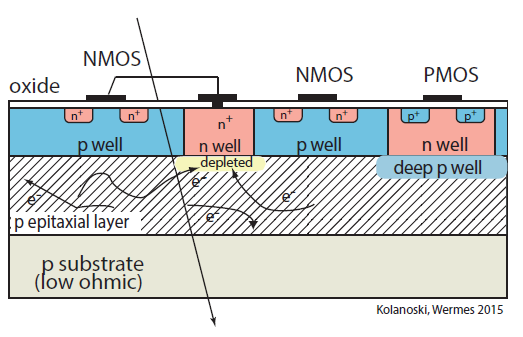
\includegraphics[scale=.7]{MAPS}
\caption{Schematic of a monolithic pixel detector (MAPS).}
\label{fig:MAPS_fig}
\end{figure}

In this detectors, not the entire area is sensitive to the charge production. Without technology modifications the sensitive layer cannot be depleted and charge collection is mostly achieved by diffusion, leading to a suboptimal charge collection efficiency. The collection electrode is a $n^{+}$ contact in a n-well, embedded in a p-epitaxial layer placed on top of a p substrate. Other n-wells can be necessary, for example, to host PMOS transistors, and for this reason they have to be shielded by deep p-well, to prevent them from becoming competitive for charge collection. These highly doped deep layers assume a negative potential with respect to the collection electrode and hence a repulsive effect.
Due to the absence of a drift field in the epi-layer, with the exception of the region immediately below the collection electrode, collection charge occurs mainly by diffusion and thus it is slow and incomplete. 
Typical values of the epi-layer thickness are within the range of 1 - \SI{20}{\micro m} \cite{Garcia-Sciveres:2017ymt}.

These MAPS detectors cannot be used in high rates experiments because they have charge collection time on the order of \SI{100}{ns}, thus too slow. The signal is very small (typically $\geq$ 1500 $e^{-}$) in this standard process, due to the small thickness of the epitaxial layer, not even fully depleted, and they also have limited radiation tolerance. The very small electrode capacitance allows the production of a sizeable signal even with a very small collected charge.
In addition, due to Non-Ionising Energy Loss (NIEL) effects \cite{wermes_book2020}, radiation produces displacement damage in the sensor bulk also creating energy levels in the band gap that act as trapping centers. 
Electrons and holes can be trapped and then be released again after some time, producing a decrease of the signal amplitudes if the de-trapping time constant is longer than the time of signal formation. 

Although their limited radiation tolerance MAPS sensors have been successfully employed for heavy ions collisions, like STAR experiment at RHIC (Relativistic Heavy Ion Collider) \cite{Greiner:2013tva} and the ALICE upgrade at the LHC \cite{ALICE:2013nwm}, which are characterized by a relatively low event rate.


\subsection{Depleted MAPS pixel detectors}

In order to obtain a fast and complete collection of the released charge, it is necessary to drift the carriers toward the electrodes by an external electric field. A full depletion of the sensitive region enhances the charge collection, producing larger signals and a better signal-to-noise ratio. \\
The depletion depth depends on the substrate resistivity and the bias voltage, according to the relation:
\medskip
\begin{equation}
d \propto \sqrt{\rho V}
\end{equation}

For this reason, new processing techniques have been employed, allowing the application of higher voltage, and/or high-resistivity substrate wafers have been used. Both techniques are used to increase the depletion region underneath the collection electrode (typically to 25– \SI{150}{\micro m}) thus providing a sufficiently large and fast signal.

We can distinguish two main variants of DMAPS pixel detectors \cite{Garcia-Sciveres:2017ymt}: with a \textit{large} or \textit{small} collection electrode, shown in~\autoref{fig:fill_factor}.

\begin{figure}[h!]
\centering
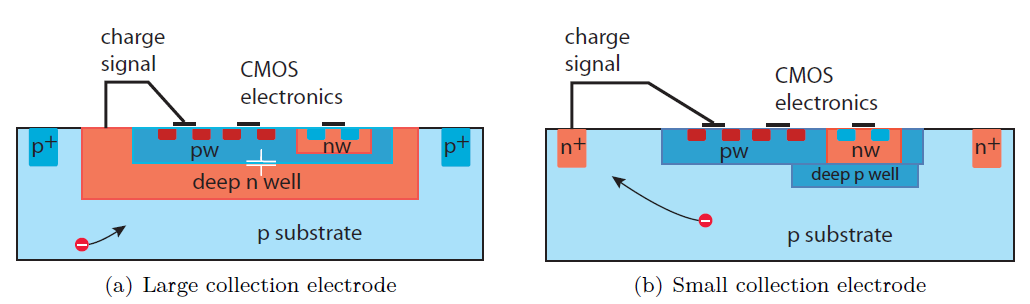
\includegraphics[scale=.6]{fill_factor}
\caption{On the left (a) a schematic of the large electrode design. On the right (b) the small electrode design.}
\label{fig:fill_factor}
\end{figure}

The \textit{large collection electrode} DMAPS features a deep n-well acting as an electrode but also as a shield for the entire CMOS readout electronics, embedded within it. With a large electrode charge is drifted vertically towards the electrode from the region underneath. This architecture improves the radiation tolerance because the reduced average drift distance of the charge carriers decreases the probability of trapping. At the same time though, the large size of the electrode implicates higher values of capacitance (several hundred fF) which increases the noise and worsens the timing performance.\\
The \textit{small collection electrode} variant has a small n-well collection node, distanced from the CMOS circuitry which is embedded in p-well and deep p-well layers needed for shielding. In this design, low capacitance of about 5-\SI{20}{fF} can be obtained, improving noise and timing performance.
Radiation tolerance instead, is more difficult to reach due to larger average distance travelled by the carriers. In addition, obtaining complete charge collection efficiency is more difficult. Smaller pixel dimensions are preferred for small electrode (to reduce the path), and therefore higher power density is accepted in exchange of increased robustness against radiation.\\


\begin{figure}[h!]
\centering
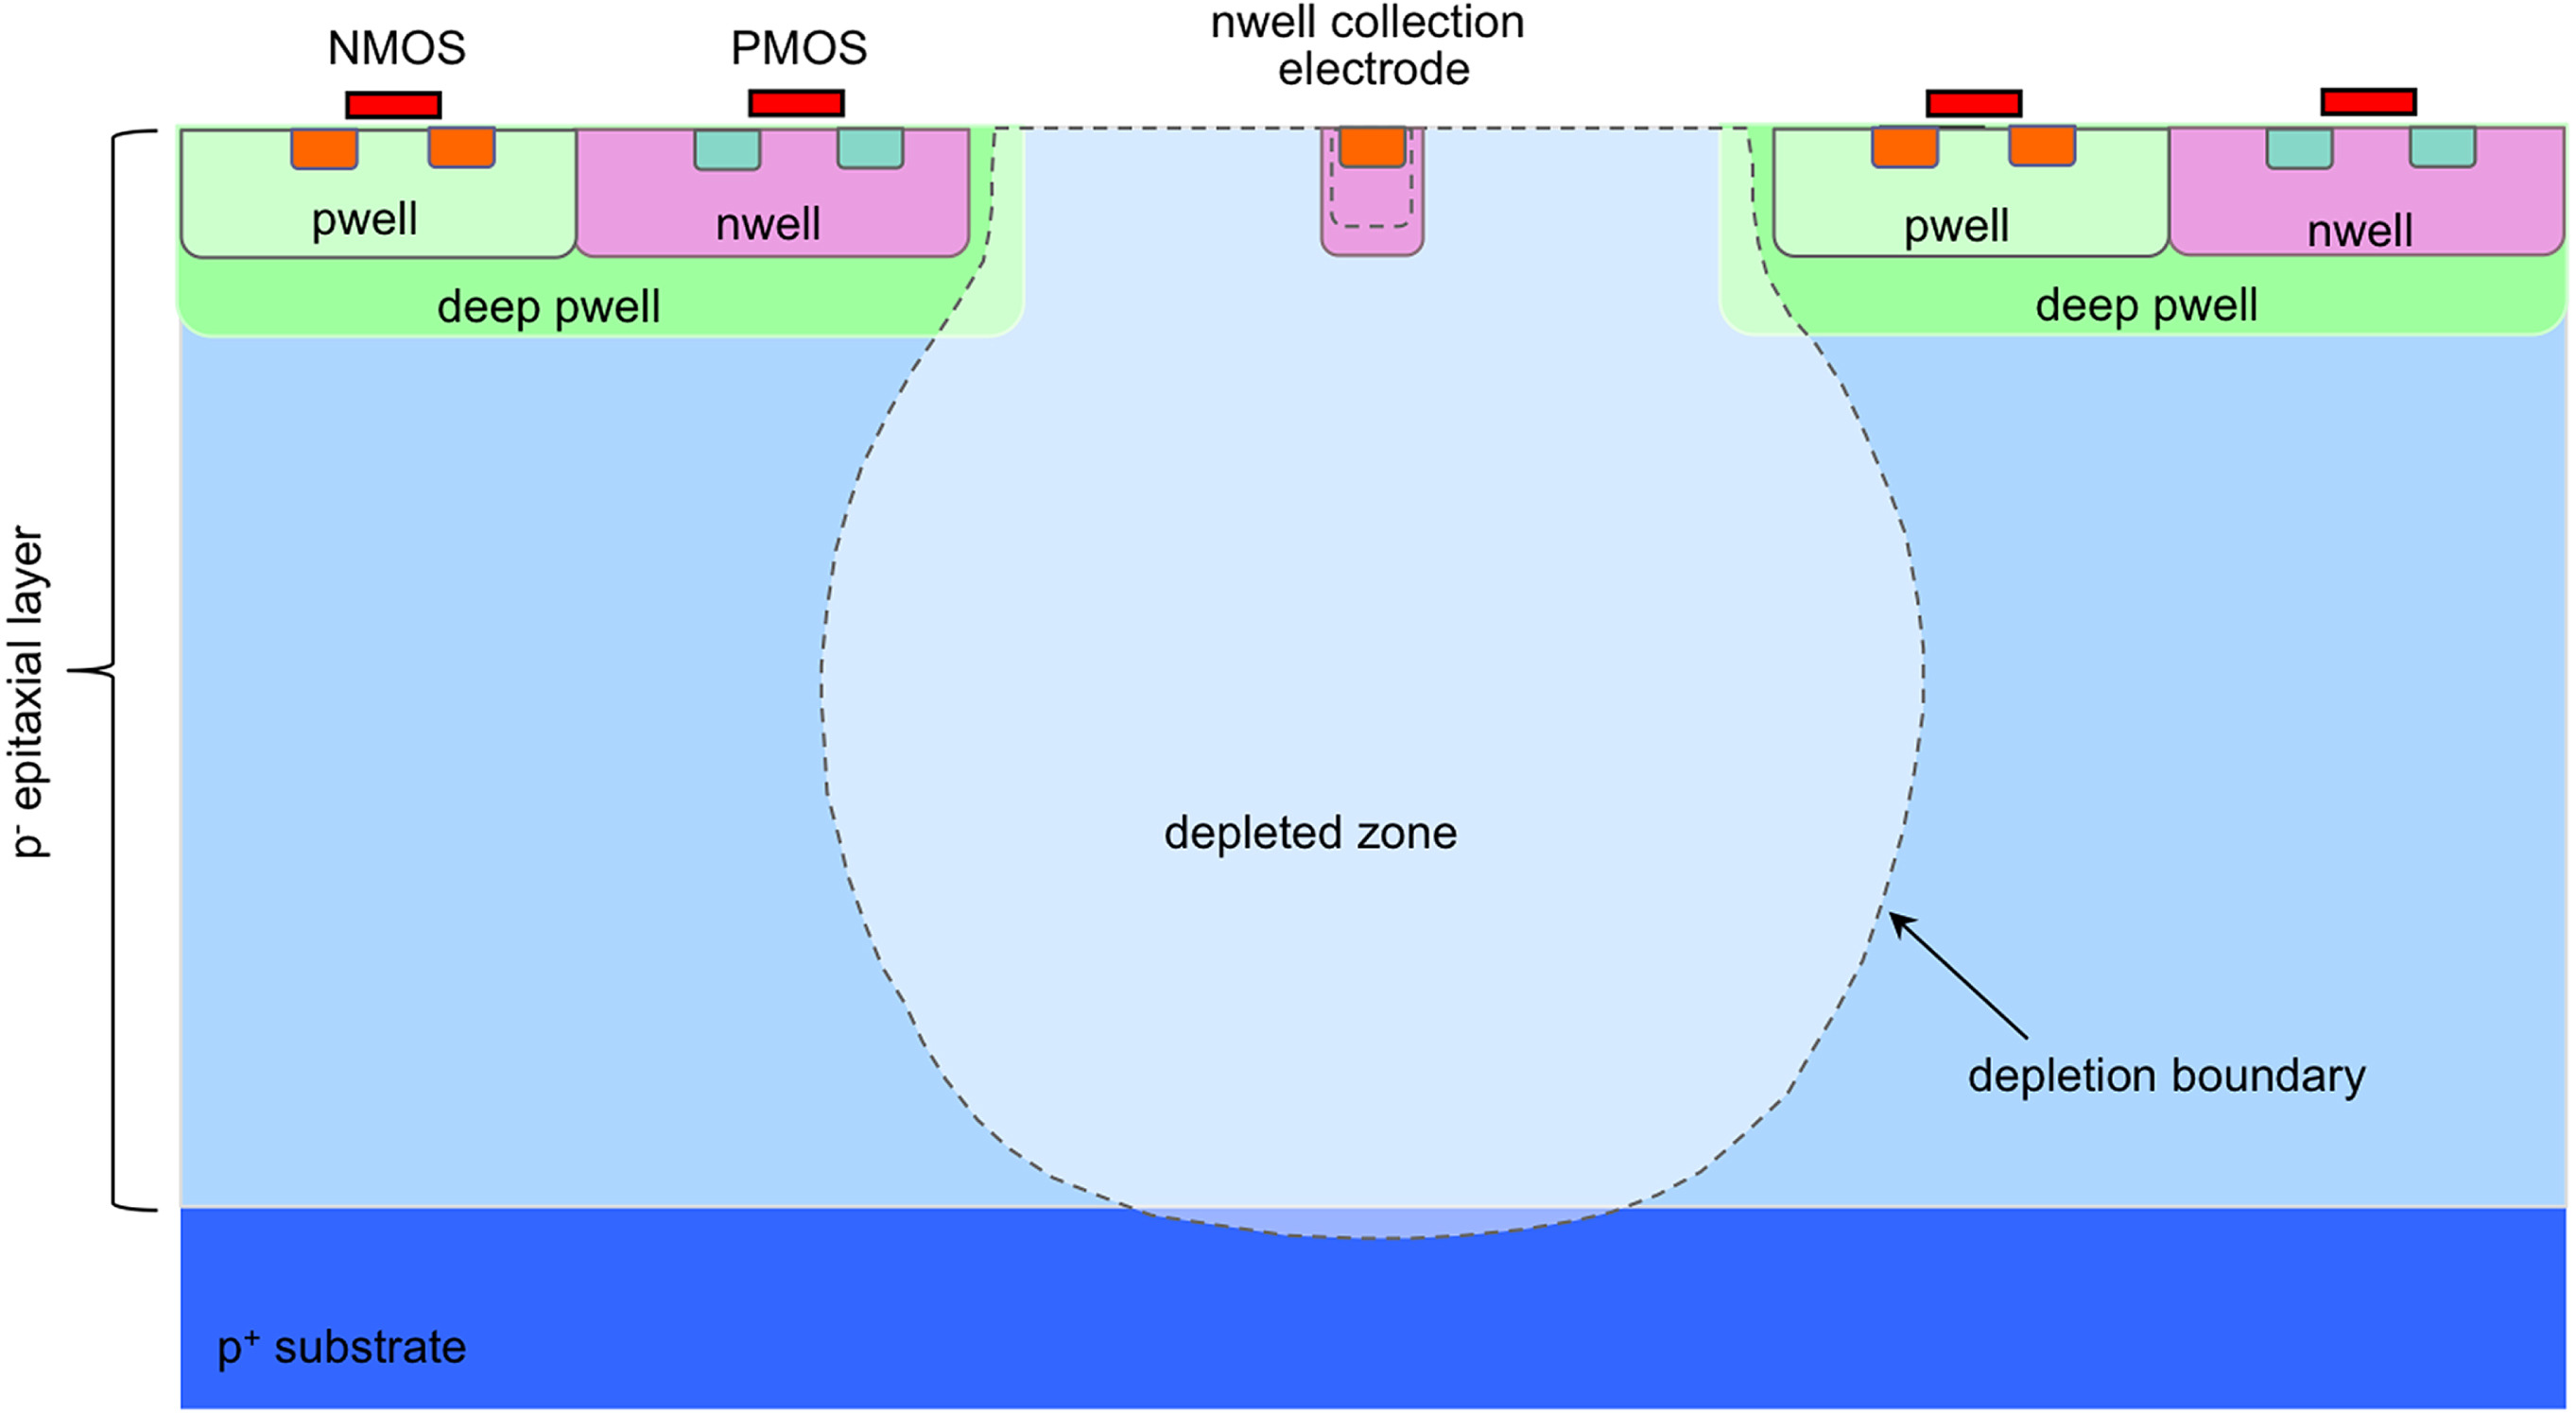
\includegraphics[width=.45\textwidth ,keepaspectratio] {alpide_process.jpg}
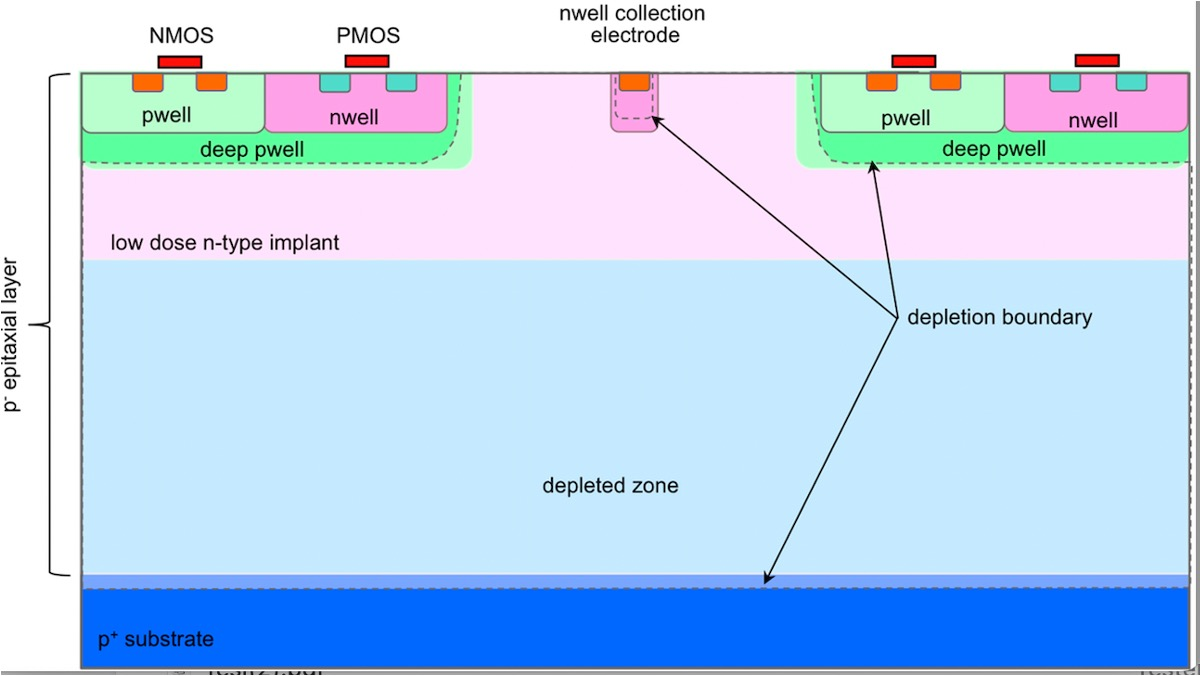
\includegraphics[width=.45\textwidth ,keepaspectratio]{modified_process.jpg}
\caption{Small electrode design adopted in the ALPIDE sensor with the standard process (left) and the process modification with the addition of a low dose n-doped layer used to implement a planar junction and deplete the epitaxial layer over the full pixel area.}
\label{fig:n_doped}
\end{figure}


In the process adopted for the ALPIDE sensor with a small electrode \cite{AGLIERIRINELLA2017583}, it is difficult to deplete the epitaxial layer over its full width as it is shown in~\autoref{fig:n_doped} left side. 
In order to achieve the full depletion of the sensitive layer, combined with a low capacitance collection electrode, a planar junction separated from the small collection electrode has been implemented.  A low dose deep n-type implant has been used to realize a planar junction in the epitaxial layer within the pixel matrix below the wells containing circuitry, as shown in~\autoref{fig:n_doped} right side. 
The epi-layer is thus depleted through two pn junctions: the deep p-wells to low dose n-implant junction, and the n-implant to p-epitaxial layer~\cite{SNOEYS201790}. This addition creates a potential minimum for electron collection underneath the deep p-well with a field direction towards the n collection well, thus strengthening the lateral collection of charges \cite{wermes_book2020}. The epi-layer is \SI{25}{\micro m} thick and the collection electrode is on positive potential.
This modification of the technology has allowed to further improve radiation tolerance. \\

The most probable value (MPV) of the signal released by a Minimum Ionizing Particle (MIP) in the thin MAPS sensitive thickness ($\approx$ \SI{25}{\micro m}) is only about 2000~$e^{-}$. 

The small charge signal achieved in the thin epi-layer (typically 1600~$e^{-}$) becomes a sizable voltage signal (about \SI{50}{mV}) due to the small ($\geq$\SI{5}{fF}) capacitance according to dV~=~dQ/C. Therefore voltage (rather than charge) amplification is employed for the readout of small electrode MAPS.



\subsection{Silicon On Insulator (SOI) technology}\label{sec:SOI_tech}

\textit{Silicon on Insulator} (SOI) technology represents another way to combine the sensitive region and the readout circuit in a single monolithic unit. In this architecture, the transistor is isolated by vertical trenches and is divided from the bulk by a \ch{SiO_{2}} layer, called \emph{buried oxide} (BOX).
An high resistivity bulk wafer allows to deplete the volume in the region below the BOX, to generate a large charge signal when a particle passes through the detector. The bulk and the CMOS electronics are connected by vertical connections, called \textit{vias}. In~\autoref{fig:SOI_fig} a monolithic SOI pixel is displayed, with a doped volume placed between the CMOS circuitry and the BOX. This variation prevents the capacitive coupling from the substrate into the electronics, through the BOX.
The SOI process is significantly more complicated than the DMAPS process, and in addition it has significant limitations in terms of radiation hardness, since under irradiation a large fixed charge accumulates in the thick oxide altering the electric fields in both the electronics and the sensor \cite{Battaglia:2009qu}.

\begin{figure}[h!]
\centering
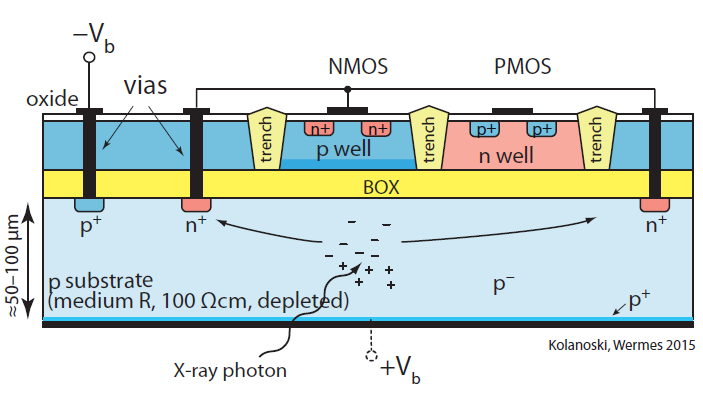
\includegraphics[scale=.7]{SOI_fig}
\caption{An example of a Monolithic SOI pixel.}
\label{fig:SOI_fig}
\end{figure}


\section{History of Monopix developments}

In recent years, requirements for high-energy physics experiments with high rates and high radiation environments have led to advances in CMOS technologies, and the development of a new generation of monolithic pixel sensors (DMAPS) with fast readout and high radiation tolerance.

Specifically two different DMAPS development lines have been followed, distinguished by different pixel architectures, using two different implementation process technologies \cite{Bespin:2020hge}:

\begin{itemize}
\item \textbf{large fill factor} line: with large collection electrode and the electronics inside the charge collection well, these prototypes are indicate to experiments with high rate and high radiation conditions, because they could ensure a greater tolerance to large doses of radiation. They have been fabricated in LFOUNDRY \SI{150}{nm} process \cite{Barbero:2019bkw}. In~\autoref{fig:LF} some of these chip developments are shown.
\item \textbf{small fill factor} line: with small collection electrode and the electronics outside the charge collection well, these devices need a process modification to enhance the radiation hardness \cite{SNOEYS201790}. They are faster compared to the previous type, and due to the smaller values of total capacitance, they require much less power consumption. They are fabricated in a TowerJazz \SI{180}{nm} CMOS imaging process, modified to include the additional implant shown in~\autoref{fig:n_doped}.
\end{itemize}

\begin{figure}[h!]
\centering
\subfigure[CCPD\_LF]
{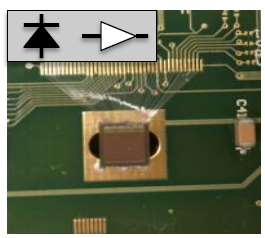
\includegraphics[scale=0.6]{LF1}}\quad
\subfigure[LF-CPIX]
{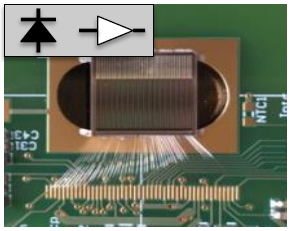
\includegraphics[scale=0.6]{LF2}}\quad
\subfigure[LF-MONOPIX 1]
{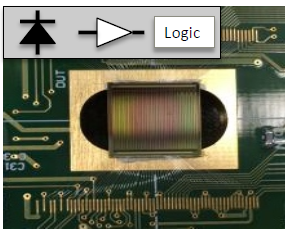
\includegraphics[scale=0.6]{LF3}}\\
\caption{LFOUNDRY \SI{150}{nm} development line.}
\label{fig:LF}
\end{figure}


\subsection{TJ-Monopix line} \label{sec:TJ}

In~\autoref{fig:TJ} the TowerJazz development line is displayed, that have led to the design of the last iteration of this series, the TJ-Monopix2 chip, whose characterization results will be shown in~\autoref{ch:TJ2}.\\

\begin{figure}[h!]
\centering
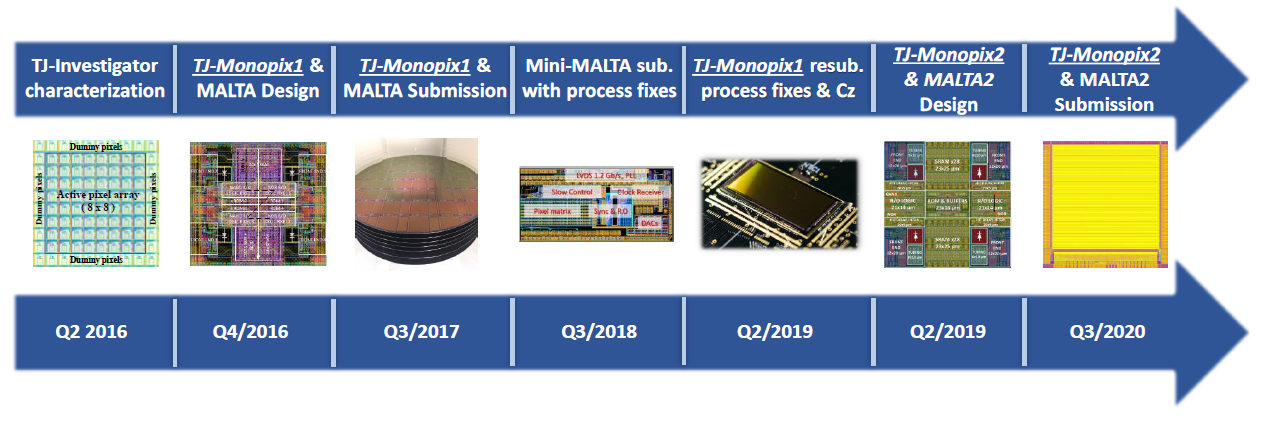
\includegraphics[scale=.55]{TJ}
\caption{TowerJazz \SI{180}{nm} development line.}
\label{fig:TJ}
\end{figure}

The standard TowerJazz \SI{180}{nm} process has been employed to realize the ALPIDE monolithic active pixel sensor, selected for the ALICE Inner Tracking System (ITS) upgrade \cite{ALICE:2013nwm, Kim:2016ktw}.

The chip proved to be suitable for the ALICE requirements, but the standard process does not ensure the full depletion volume, which is crucial to limit the signal degradation especially after irradiation. For this reason, the aforementioned process modification have been developed by CERN in collaboration with the foundry \cite{SNOEYS201790}, that allows full depletion of the sensitive layer. This new implementation has been tested in a dedicated chip called TJ-Investigator \cite{AglieriRinella:2020rcb}, and the results obtained have demonstrated the effectiveness of the modified process. \\
Therefore two large scale demonstrator chips have been realized, called TJ-Monopix1 and TJ-Malta1 \cite{Moustakas:2017qqw}, whose main difference lies in the readout architecture. The TJ-Malta1 chip implemented an \textit{asynchronous} readout architecture, which eliminate the Bunch Crossing ID (BCID, timestamp), to reduce the digital power consumption. For TJ-Monopix1 instead, a \textit{coulmn-drain} readout architecture was chosen, which will be described in the following, as it is the same implemented in TJ-Monopix2. Both chips have been fully tested and irradiated to investigate their functionality and efficiency, which however has decreased from 97\% to 70\% after irradiation with an equivalent neutron fluence of \SI{e15}{n_{eq}/cm^{2}} \cite{Caicedo:2019lrk}. 

\begin{figure}[h!]
\centering
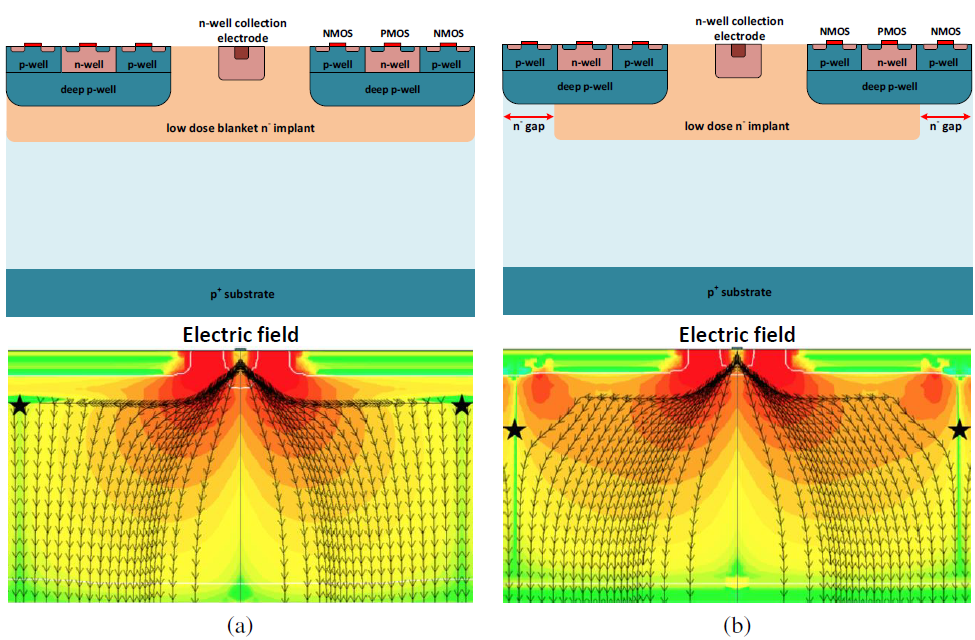
\includegraphics[scale=.7]{enhance_lateral}
\caption{On the left, the lateral electric field for a pixel implementation in the modified process (only low dose n$^{-}$ implant), compared with the modified process with the n-gap variant.}
\label{fig:enhance_lat}
\end{figure}


The main reason for the efficiency drop has been discovered to be related to the weak lateral electric field at the pixel edges. So the process has been further optimized to resolve this issue. Two different approaches were found to increase the lateral electric field at the pixel borders~\cite{Munker_2019}: creating a gap in the deep n-implant \textbf{n-gap} variant, requiring only a mask change, or introducing an additional p-type implant at the pixel border \textbf{extra deep p-well} variant. The n-gap variant is shown in~\autoref{fig:enhance_lat} compared to the previous version.

It can be seen the significant improvement of the electric lateral field, which results in turn in faster charge collection and high efficiency even after irradiation. 

Further optimization of the pixel size, which is critical to take full advantage of field shaping through process modifications and to improve charge collection, have been implemented in the last iteration of this development line: TJ-Monopix2, considered as starting point for the development of the OBELIX final chip, designed for the upgrade of the Belle II vertex detector.


\subsection{TJ-Monopix2 architecture}\label{sec:TJ_arch}

We will briefly describe the chip architecture of TJ-Monopix2. 

\begin{description}
\item[Analog front-end]
\end{description}

The advantage of the small collection electrode concept is the small capacitance, which allows to transform the charge signal arriving on the sensing node into a high voltage signal (dV~=~dQ/C).

In~\autoref{fig:analog} a schematic of the voltage amplification and the readout stages is shown.

\begin{figure}[h!]
\centering
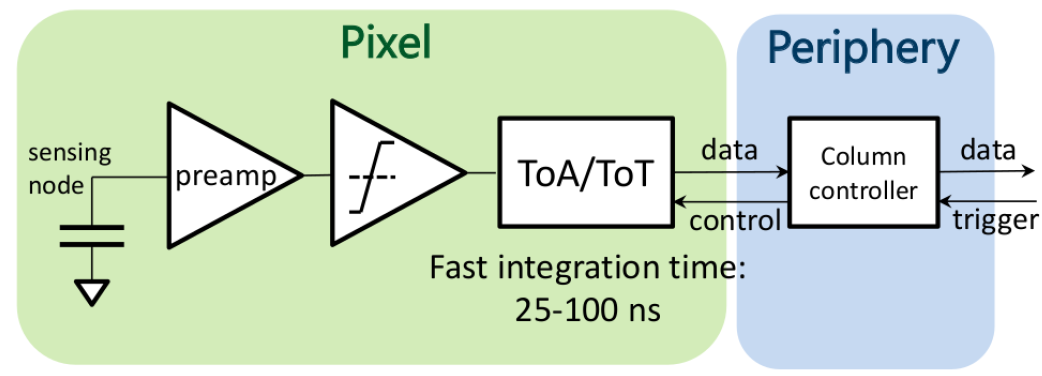
\includegraphics[scale=.5]{analog2}
\caption{Sketch of the voltage amplification stages and the readout.}
\label{fig:analog}
\end{figure}

The charge signal, produced by particles traversing the sensor and collected by the collection node, is converted in a voltage signal through a small capacitance. It goes to a pre-amplifier and then to a discriminator, providing a digital output signal when the input is above the set threshold. The length of the output signal is the Time Over Threshold (TOT) and provides also information about the signal charge. 
The pre-amplifier and the discriminator working conditions are defined by several chip registers (as we will see in \autoref{ch:TJ2}). The collected data are finally sent to the chip periphery in order to transmit and store them outside the chip.\\


\begin{figure}[h!]
\centering
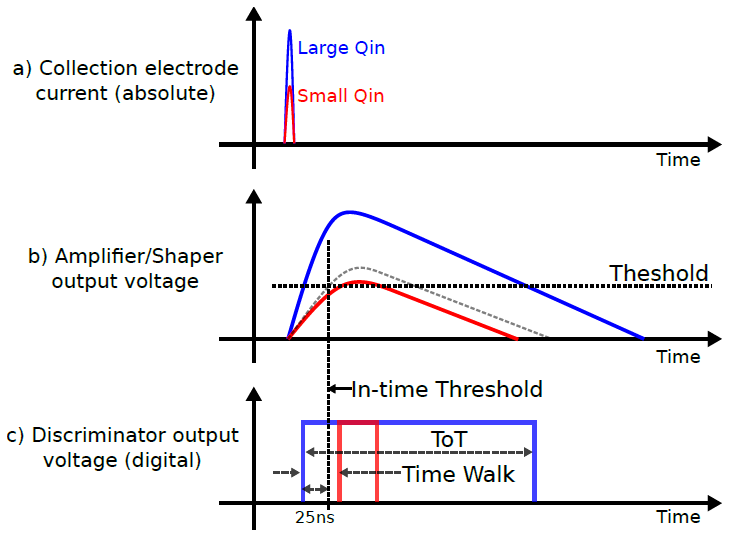
\includegraphics[scale=.7]{ToT}
\caption{Time Over Threshold (TOT) technique.}
\label{fig:tot_scheme}
\end{figure}

\begin{description}
\item[The column-drain readout architecture]
\end{description}

The readout architecture \cite{Moustakas:2018ure, Moustakas:2021gjr} implemented in TJ-Monopix ensures fast readout by encoding the analog charge information using the standard Time Over Threshold (TOT) technique shown in~\autoref{fig:tot_scheme}. This procedure exploits two timing information: the \textit{Leading Edge} (LE) which corresponds to the hit time of arrival (when the signal value goes over the threshold), and the \textit{Trailing Edge} (TE) that is when the signal goes below the threshold value. From the difference between the TE and the LE, the TOT can be calculated.\\

The \textit{in-pixel} circuitry implements a Random Memory Access (RAM) to store the LE and TE timing info, a Read-Only Memory (ROM) to store the pixel address and the control and arbitration logic, essential to read out the hit, as described in the following.
 
The readout is \textit{column-based}, so all pixels of each double column share a common column-bus which could be accessed by one pixel at a time, with a defined priority logic. The column bus includes the BCID timestamp, the data (LE, TE, address) and the control signals.
The \textit{periphery} includes the End Of Column (EoC) block which deals with the transmission and the readout of the column-bus signals, and the Digital Chip Bottom (DCB) that instead, processes the hit information. The overall scheme of TJ-Monopix2 is shown in~\autoref{fig:RO}. 

\begin{figure}[h!]
\centering
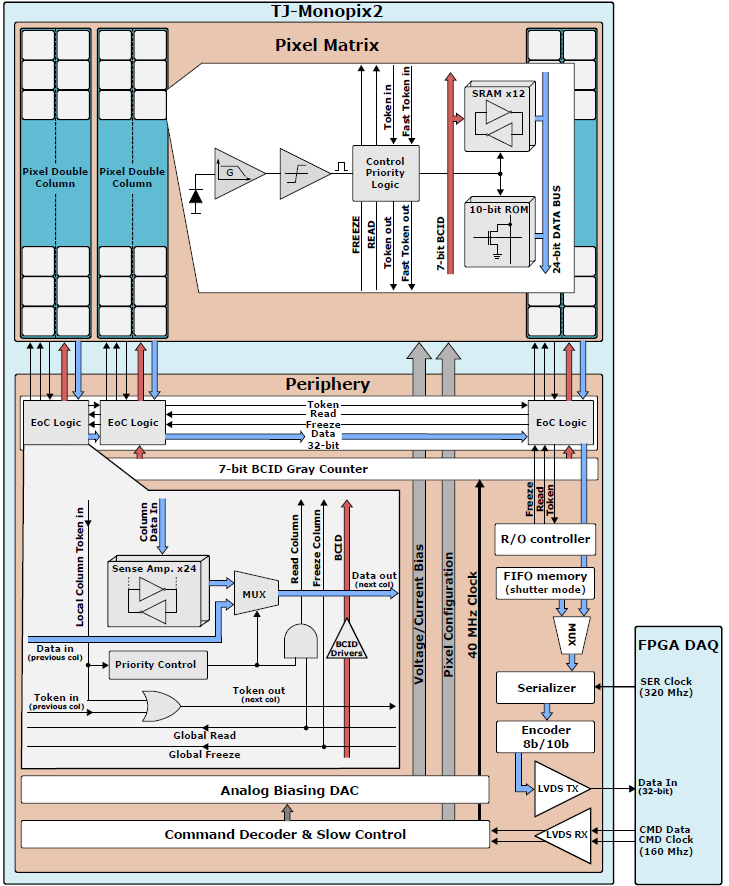
\includegraphics[scale=1]{RO}
\caption{Architecture of TJ-Monopix2.}
\label{fig:RO}
\end{figure}

\begin{comment}
The readout could be triggered or full-readout. In TJ-Monopix line hit data is continuously transmitted to the DAQ. In case of triggered readout instead, hit data is stored in a trigger memory, and the information is transmitted only when the trigger signal arrives.
\end{comment}

%%%%%%%%%%%%%%%%%%%%%%%%%%%%%%%%%%%%%

The column-drain architecture uses a \textsc{token} signal interpreted by the pixel control logic when data are available to be readout. Only pixels with a non-zero signal are readout, when going through a column, realizing an on-chip sparsification mechanism that allows fast readout. No local buffer is implemented, so a hit pixel remains frozen, and therefore insensitive, until it is readout.

\begin{figure}[h!]
\centering
\subfigure[Schematic of TJ-Monopix2 in-pixel readout logic.]{
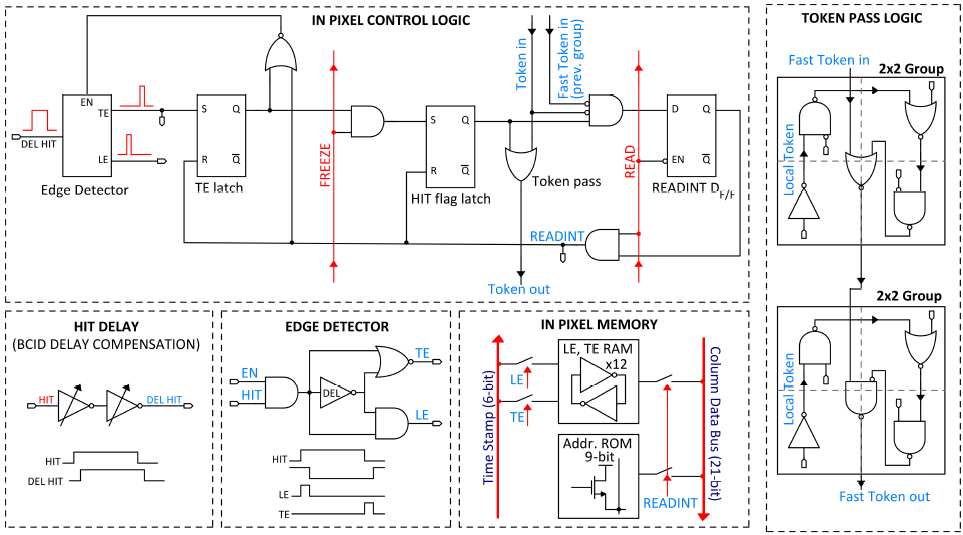
\includegraphics[scale=.8]{inpixel_ro}}\\
\subfigure[Simulation of the in-pixel readout logic.]{
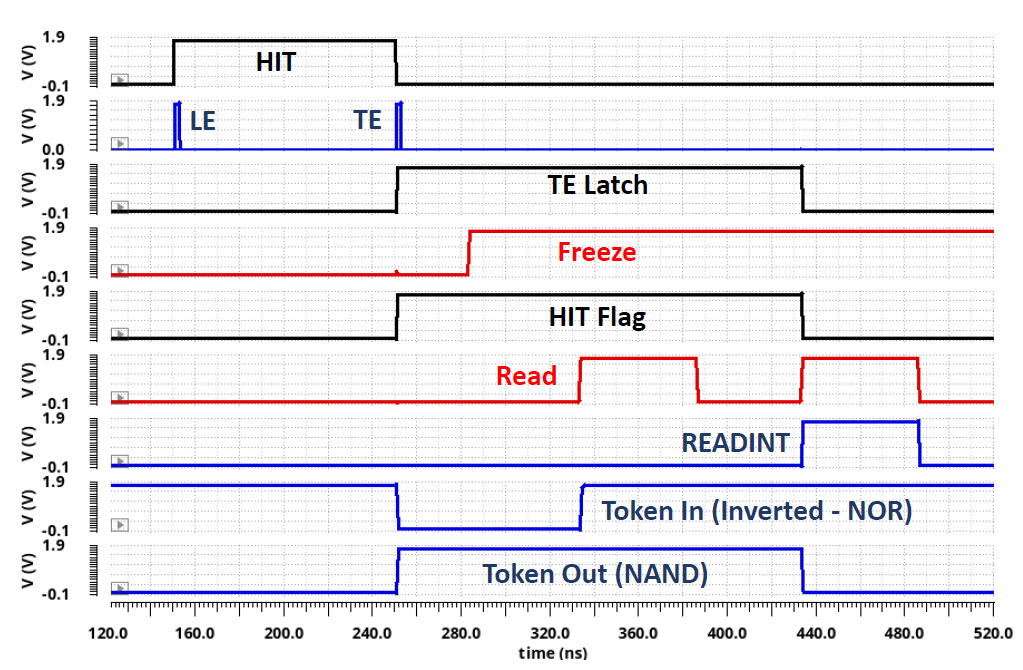
\includegraphics[scale=.6]{inpixel_ro_sim}}
\caption{}
\label{fig:inpixelro}
\end{figure}

\begin{comment}
\begin{figure}[h!]
\centering
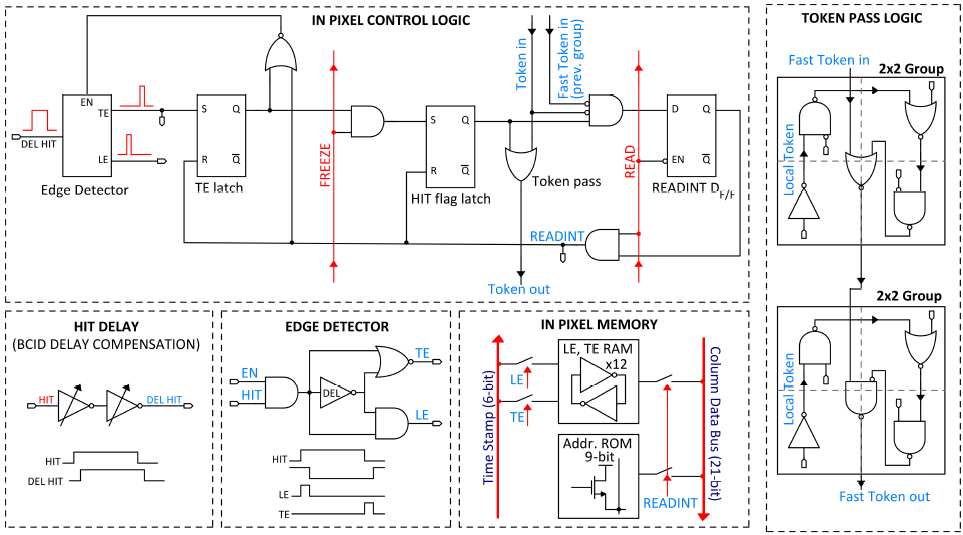
\includegraphics[scale=.8]{inpixel_ro}
\caption{Schematic of TJ-Monopix2 in-pixel readout logic.}
\label{fig:inpixelro}
\end{figure}
\end{comment}



%\\
The schematic and a simulation of the in-pixel readout logic are shown in~\autoref{fig:inpixelro}.
The digital output signal coming from the FE is transmitted to an edge detector which generates the TE and LE pulses. The TE and LE pulses force the storage of the current timestamp (6 bits) into a 12 bit memory cell. The TE signal is sent to an SR latch, which registers the hit and disables the edge detector, preventing new hits to be registered before reading out the previous one. 
If the column is not frozen, a HIT flag latch is activated, which signals the presence of the hit to be readout. This latch also activates the \textsc{token} signal which informs the readout controller that hits could be read. In TJ-Monopix2 two \textsc{token} signals are implemented: a fast one, which, taking advantage of pixel grouping in \numproduct{2 x 2} cores, defines the higher (group) level priority and propagates across the
double column; and a local one, which defines the priority within the group. When the readout controller receives the information from the \textsc{token}, the matrix is frozen by asserting the \textsc{freeze} signal. 
Then the \textsc{read} signal is raised and data (TE, LE, pixel address information) are transmitted to the periphery through the column data-bus, accessible only if the \textsc{token} signals allow it (highest priority) and the HIT flag is active. In this case, the raising edge of the \textsc{read} enables a D-latch and at the same time, resets the TE and the HIT flag latches. In the meantime, if the D-latch is set and enabled by the \textsc{read}, an internal signal, called \textsc{readint} is produced to control the access of the data to the column data-bus.\\

In conclusion the main features of the TJ-Monopix2 architecture can be summarized as follows:

\begin{itemize}
\item the chip is self-triggered and the hit pixels are frozen by the first pixel that completes the TOT cycle;
\item each pixel stores its own address and the timestamps of the leading and trailing edges of the TOT;
\item a token-passing logic is implemented to read the data from only the hit pixels without wasting clock cycles;
\item while the readout is proceeding the free pixels can still store their TOT, but will be readout in a successive read cycle.
\end{itemize}


\begin{comment}
In~\autoref{fig:RO2} is displayed an example of the readout of two hits. 

\begin{figure}[h!]
\centering
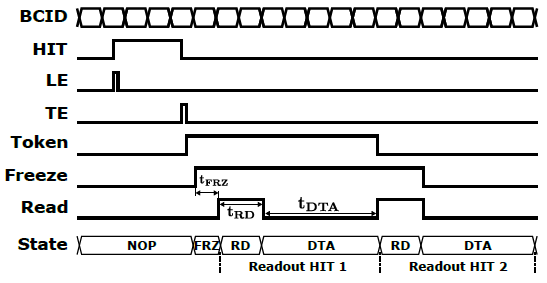
\includegraphics[scale=1]{RO2}
\caption{Schematic of a readout sequence where two hits are being processed.}
\label{fig:RO2}
\end{figure}
\end{comment}
